
\section{Section title}
\label{sec-1}
For bibliography use \cite{RefJ}
\subsection{Subsection title}
\label{sec-2}
Don't forget to give each section, subsection, subsubsection, and
paragraph a unique label (see Sect.~\ref{sec-1}).

For one-column wide figures use syntax of figure~\ref{fig-1}
\begin{figure}[h]
% Use the relevant command for your figure-insertion program
% to insert the figure file.
\centering
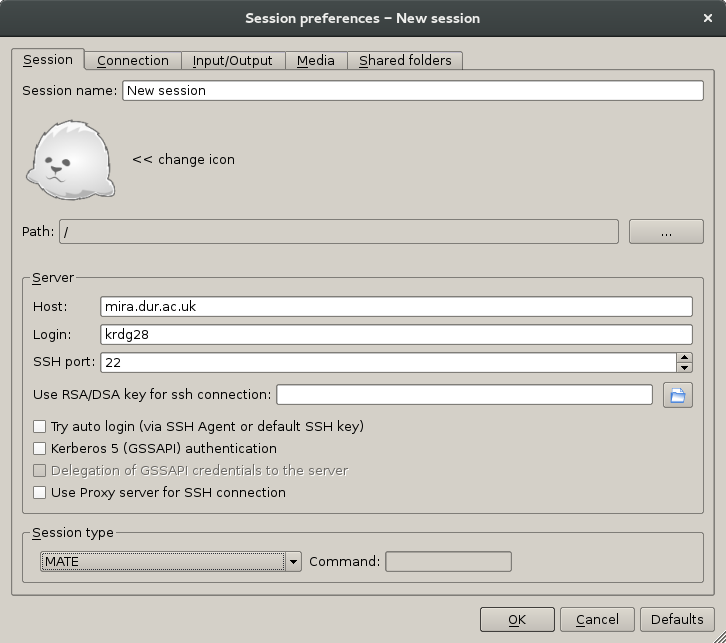
\includegraphics[width=1cm,clip]{tiger}
\caption{Please write your figure caption here}
\label{fig-1}       % Give a unique label
\end{figure}

For two-column wide figures use syntax of figure~\ref{fig-2}
\begin{figure*}
\centering
% Use the relevant command for your figure-insertion program
% to insert the figure file. See example above.
% If not, use
\vspace*{5cm}       % Give the correct figure height in cm
\caption{Please write your figure caption here}
\label{fig-2}       % Give a unique label
\end{figure*}

For figure with sidecaption legend use syntax of figure
\begin{figure}
% Use the relevant command for your figure-insertion program
% to insert the figure file.
\centering
\sidecaption
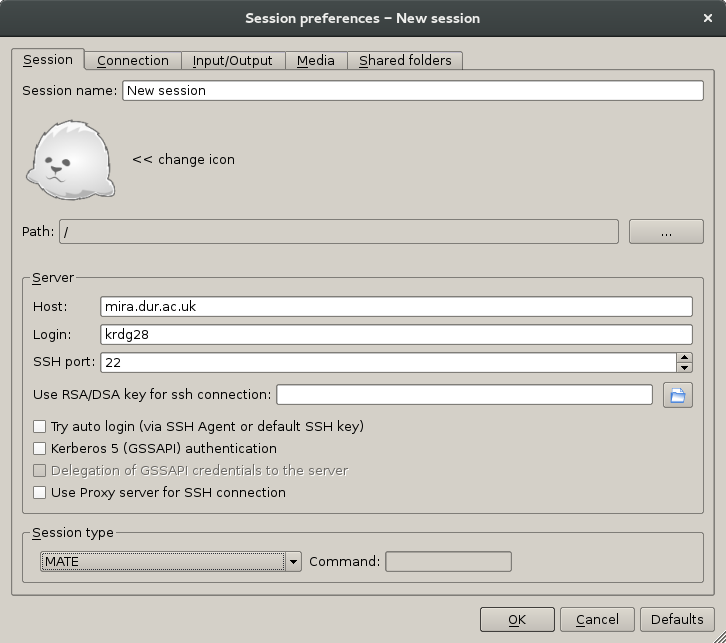
\includegraphics[width=5cm,clip]{tiger}
\caption{Please write your figure caption here}
\label{fig-3}       % Give a unique label
\end{figure}

For tables use syntax in table~\ref{tab-1}.
\begin{table}
\centering
\caption{Please write your table caption here}
\label{tab-1}       % Give a unique label
% For LaTeX tables you can use
\begin{tabular}{lll}
\hline
first & second & third  \\\hline
number & number & number \\
number & number & number \\\hline
\end{tabular}
% Or use
\vspace*{5cm}  % with the correct table height
\end{table}
